\part{Autonomous-ODEs}
\lecture{Autonomous ODEs}{Autonomous-ODEs}
\section{Autonomous ODEs}

\title{Ordinary Differential Equations}
\subtitle{Math 232 - Week 3, Day 2}
\date{12 Sep 2012}

\begin{frame}
  \titlepage
\end{frame}

\begin{frame}
  \frametitle{Outline}
  \tableofcontents[pausesection,hideothersubsections]

  Section 2.5 in book.
\end{frame}


\subsection{Solutions to DEs}


\begin{frame}
  \frametitle{What is a solution to a DE?}

  What is the solution to the DE

  \begin{eqnarray*}
    y' & = & t^2 + y^2?
  \end{eqnarray*}

  \uncover<2->{I do not know!}


\end{frame}


\begin{frame}
  \frametitle{Slope Field}

  Look at the slope field:
  \begin{eqnarray*}
    y' & = & t^2 + y^2?
  \end{eqnarray*}


  \only<1>{\includegraphics[height=5cm]{img/week3-D3SlopeExample}}
  \only<2->{\includegraphics[height=5cm]{img/week3-D3SlopeExampleSolutions}}

  Look at equilibria, stability, and look for straight line solutions.

\end{frame}


\iftoggle{clicker}{%
\begin{frame}
  \frametitle{Clicker Quiz}
    
      \ifnum\value{clickerQuiz}=1{%

        Look at the slope field:
        \begin{eqnarray*}
          y' & = & -t - y^2?
        \end{eqnarray*}

        \begin{columns}
          \column{.6\textwidth} 

          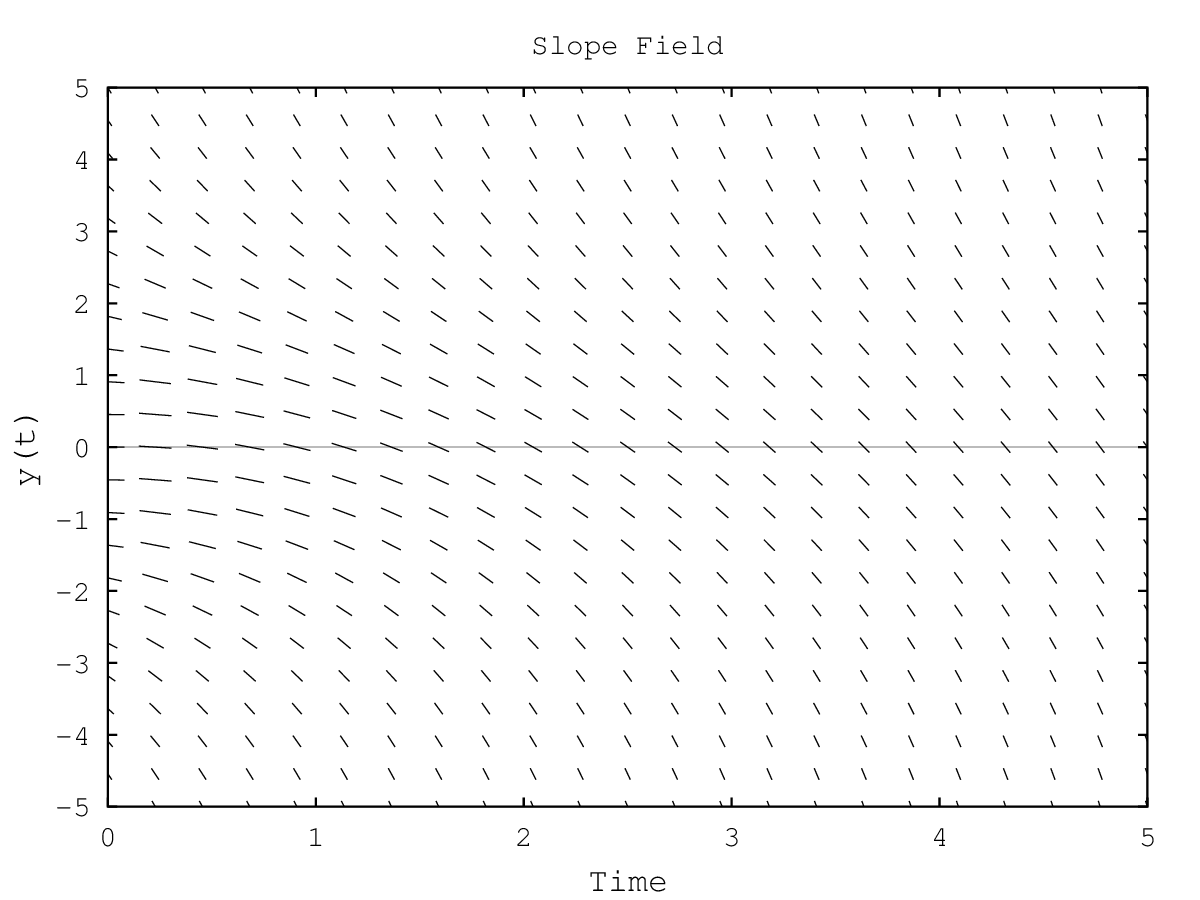
\includegraphics[height=5cm]{img/stabilityClicker1}

          \column{.4\textwidth}
          True or False: The solution to this differential equation is stable.

          \begin{tabular}{l@{\hspace{3em}}l}
            A: & True. \\
            B: & False. \\
            C: & Who knows? \\
            D: & Truth is subjective. \\ 
          \end{tabular}

        \end{columns}

     }\fi

     \ifnum\value{clickerQuiz}=2{%

        Look at the slope field:
        \begin{eqnarray*}
          y' & = & \frac{3}{2}-y?
        \end{eqnarray*}


        \begin{columns}
          \column{.6\textwidth} 

          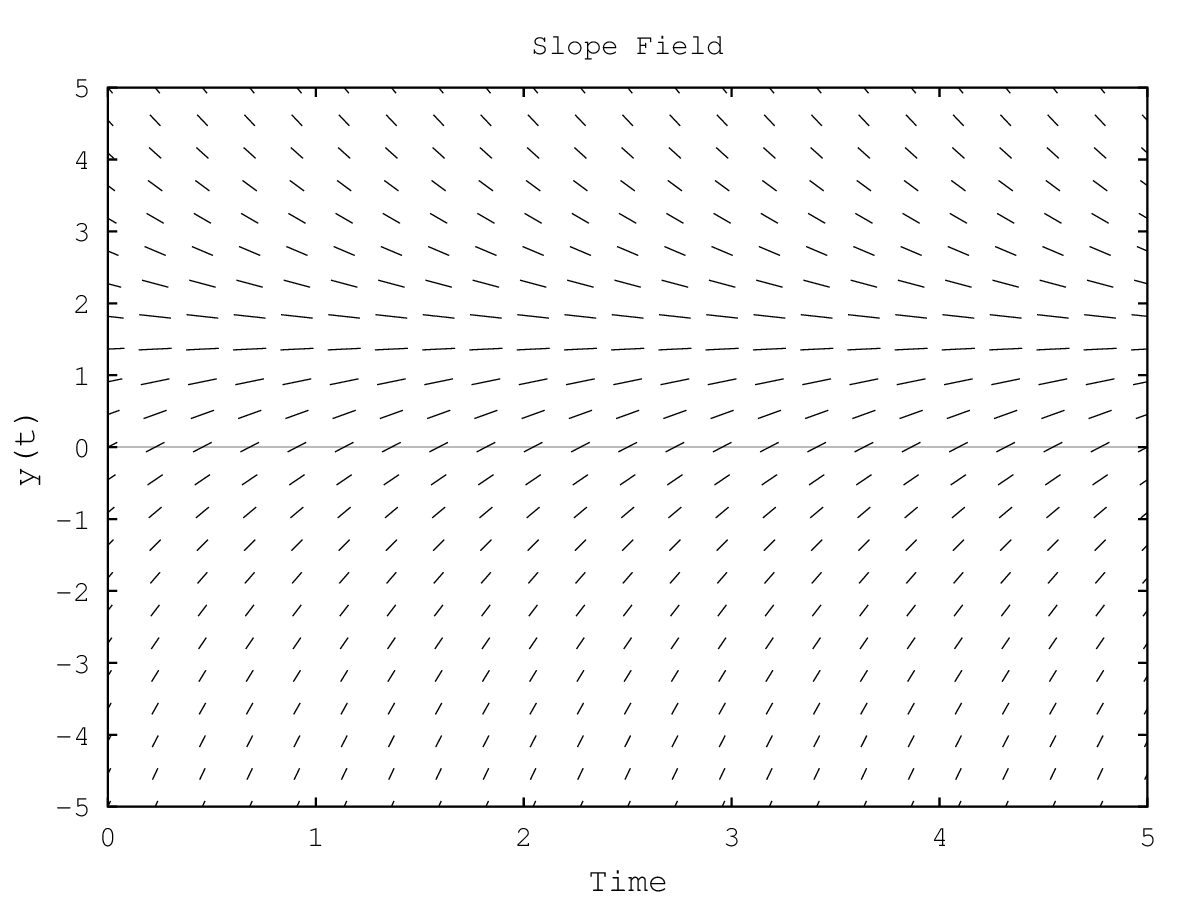
\includegraphics[height=5cm]{img/stabilityClicker2}

          \column{.4\textwidth}
          True or False: The solution to this differential equation is stable.

          \begin{tabular}{l@{\hspace{3em}}l}
            A: & True. \\
            B: & False. \\
            C: & Who knows? \\
            D: & Truth is subjective. \\ 
          \end{tabular}

        \end{columns}

     }\fi

      \ifnum\value{clickerQuiz}=3{%

     }\fi

    \vfill
    \vfill
    \vfill

\end{frame}

}


\subsection{Autonomous DEs}

\begin{frame}
  \frametitle{Autonomous DEs}

  A differential equation is \textit{autonomous} if it can be
  expressed in the form
  \begin{eqnarray*}
    y' & = & f(y).
  \end{eqnarray*}

  i.e. the DE does not have a time term explicitly given in the
  equation.


\end{frame}


\begin{frame}
  \frametitle{The slope only depends on y!}

  \vspace*{-3em}
  \begin{eqnarray*}
    y' & = & f(y).
  \end{eqnarray*}

  If the slope at $y=1$ and $t=1$ is $\half$, then it will be the same
  slope for all points where $y=1$. 

  \vfill
  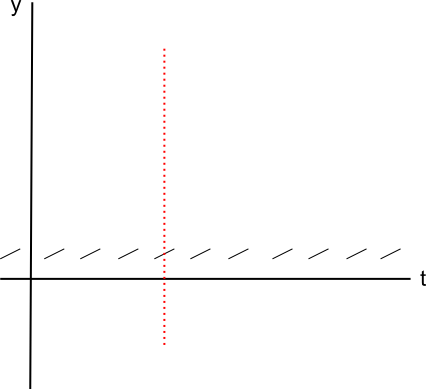
\includegraphics[width=5cm]{img/autonomousEqnSlopeField}
  \vfill

  We just need to find the slope for each value of $y$ and not worry
  about $t$.

\end{frame}

\begin{frame}
  \frametitle{The Phase Line}

  The phase line for a differential equation is a vertical line that
  indicates whether the slope is positive, negative, or zero for
  different values of $y$.
\end{frame}

\begin{frame}
  \frametitle{Example}
  \begin{eqnarray*}
    y' & = & 2y(3-y), \\
    \Rightarrow f(y) & = & 2y(3-y)
  \end{eqnarray*}


  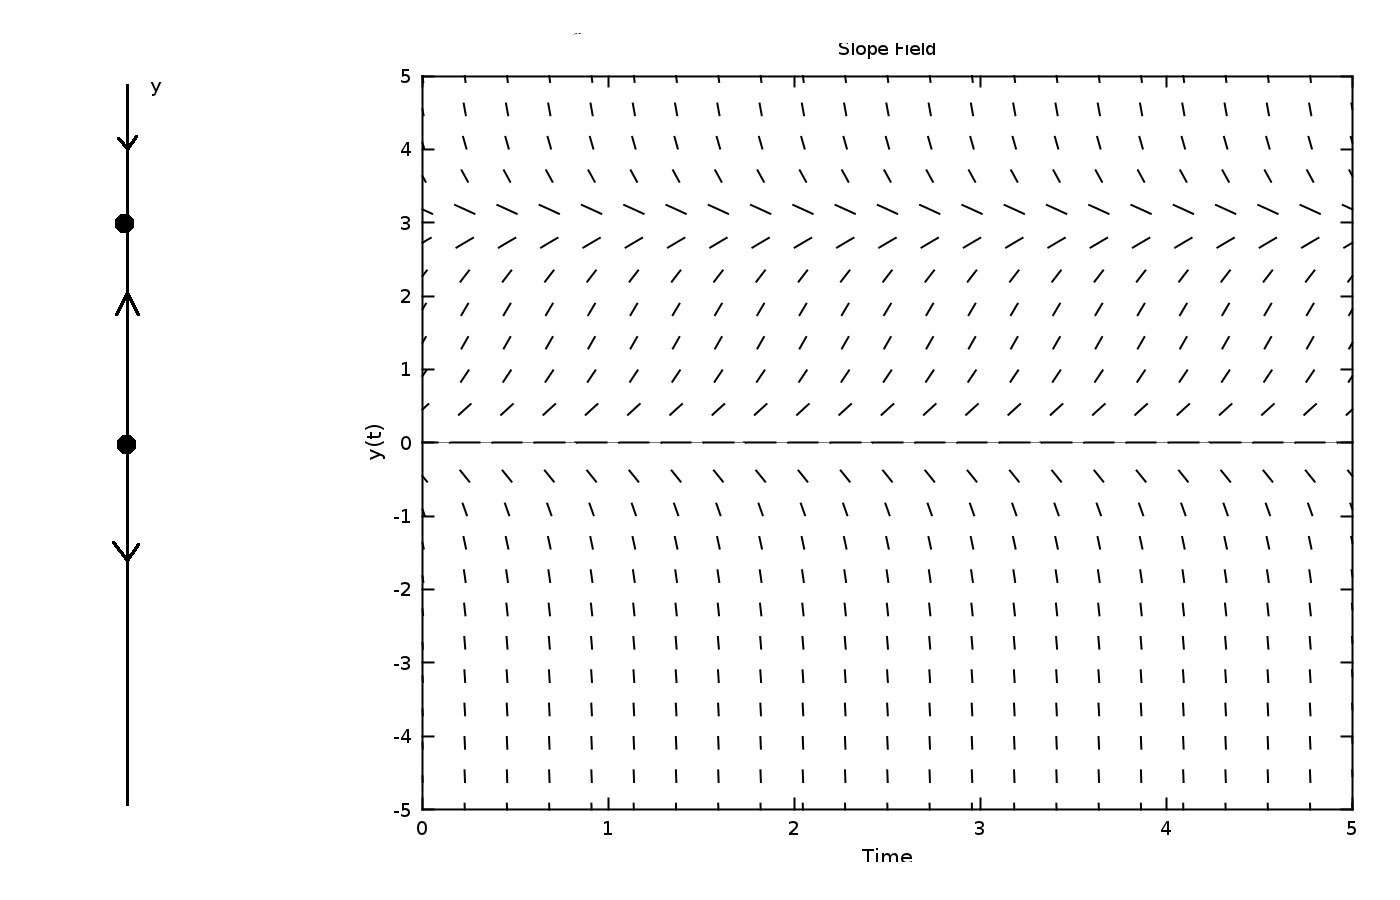
\includegraphics[height=6cm]{img/week3PhaseLineExample1}

\end{frame}


\begin{frame}
  \frametitle{Examples}
  
  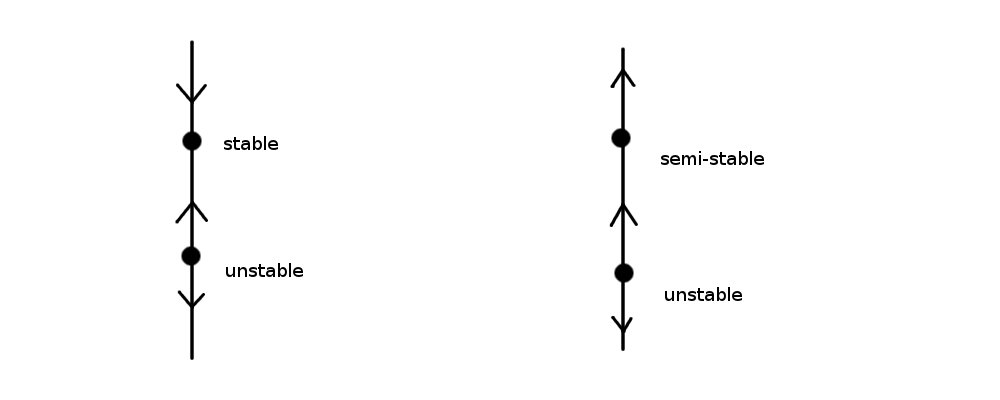
\includegraphics[height=6cm]{img/week3PhaseLine}

\end{frame}

\begin{frame}
  \frametitle{Examples}


  \begin{eqnarray*}
    y' & = & y(2-y)(4-y), \\
    \Rightarrow f(y) & = & y(2-y)(4-y)
  \end{eqnarray*}

  \begin{eqnarray*}
    y' & = & y(2-y^2), \\
    \Rightarrow f(y) & = & y(2-y^2)
  \end{eqnarray*}

  (phase lines drawn on board)

\end{frame}

\iftoggle{clicker}{%
\begin{frame}
  \frametitle{Clicker Quiz}
    
      \ifnum\value{clickerQuiz}=1{%

        Which phase line is the correct phase line for the
        differential equation
        \begin{eqnarray*}
          y ' & = & y^3-y^2
        \end{eqnarray*}

          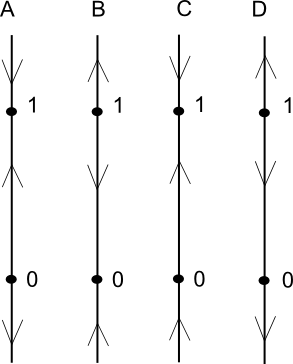
\includegraphics[height=5cm]{img/phaseLinesClickerSect1}

     }\fi

     \ifnum\value{clickerQuiz}=2{%


        Which phase line is the correct phase line for the
        differential equation
        \begin{eqnarray*}
          y ' & = & y^2 + 3y - 4
        \end{eqnarray*}

        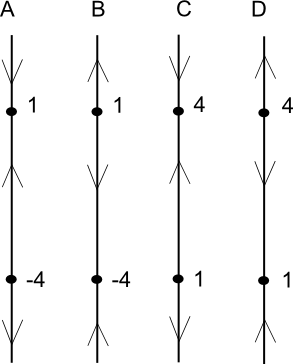
\includegraphics[height=5cm]{img/phaseLinesClickerSect2}


     }\fi

      \ifnum\value{clickerQuiz}=3{%

     }\fi

    \vfill
    \vfill
    \vfill

\end{frame}

}



\subsection{Logistic Growth}

\begin{frame}
  \frametitle{Logistic Growth}

  \vspace*{-4em}
  \begin{eqnarray*}
    y' & = & ky,
  \end{eqnarray*}
  
  If $y$ is ``small'' $k$ should be positive.

  If $y$ is ``big'' $k$ should be negative.

  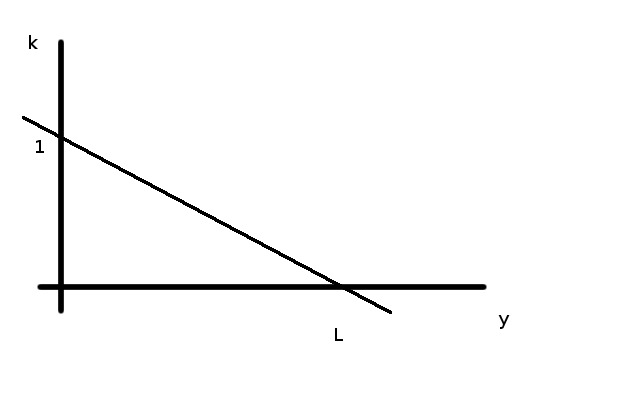
\includegraphics[height=4cm]{img/week3GrowthRate}

  Let 
  \begin{eqnarray*}
    k & = & r \lp 1 - \frac{y}{L} \rp
  \end{eqnarray*}


\end{frame}


\begin{frame}
  \frametitle{Logistic Equation}

  \begin{eqnarray*}
    y' & = & r \lp 1 - \frac{y}{L} \rp y
  \end{eqnarray*}

  Stationary points: $y=0$ and $y=L$. 

  ($L$ is called the ``carrying capacity'')

  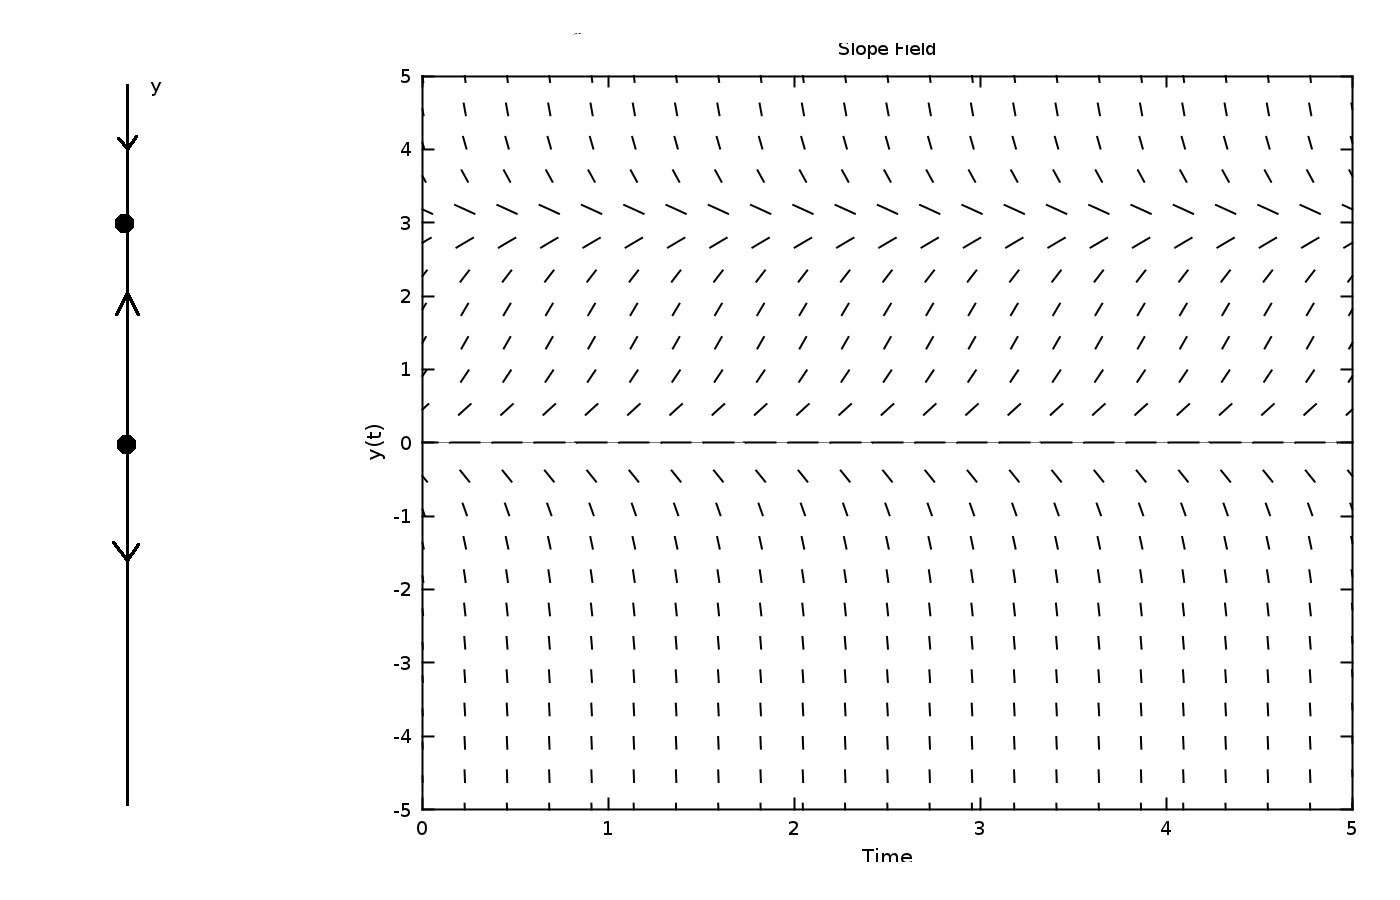
\includegraphics[height=6cm]{img/week3PhaseLineExample1}

\end{frame}


\begin{frame}
  \frametitle{Analytic Solution}

  \begin{eqnarray*}
    y' & = & r \lp 1 - \frac{y}{L} \rp y, \\
    \uncover<2->{
      \frac{y'}{\lp 1 - \frac{y}{L} \rp y} & = & r \\
      \int \frac{y'}{\lp 1 - \frac{y}{L} \rp y} ~ dt & = & \int r ~ dt       
    }
  \end{eqnarray*}

\end{frame}


\begin{frame}


  \begin{eqnarray*}
    \frac{1}{\lp 1 - \frac{y}{L} \rp y} & = & \frac{a}{1 - \frac{y}{L}} + \frac{b}{y} \\
    \Rightarrow 1 & = & a y + b \lp 1 - \frac{y}{L} \rp \\
    b & = & 1, \\
    a & = & \frac{1}{L}
  \end{eqnarray*}

    
\end{frame}

  \begin{frame}

  \begin{eqnarray*}
      \int \frac{1}{\lp 1 - \frac{y}{L} \rp y} ~ dy & = & \int r ~ dt \\
      \int \frac{1}{L} \cdot \frac{1}{1 - \frac{y}{L}} + \frac{1}{y} ~ dy & = & \int r ~ dt \\
      -\ln\lp 1 - \frac{y}{L}\rp + \ln(y) & = & rt + C \\
      \ln\lp\frac{y}{1 - \frac{y}{L}}\rp & = & rt + C \\
      \frac{y}{1 - \frac{y}{L}} & = & k e^{rt} \\
      \Rightarrow y & = & \frac{k e^{rt}}{1 + \frac{1}{L} k e^{rt}}  
  \end{eqnarray*}


  From the initial condition,
  \begin{eqnarray*}
    y(0) & = & y_0, \\
    k & = & \frac{y_0}{1 - \frac{y_0}{L}}
  \end{eqnarray*}
  

\end{frame}



% LocalWords:  Clarkson pausesection hideothersubsections
